\documentclass{../Common/Structure/doc_pdf}

\usepackage{alloy}

\titleSubtitle{{\Huge\textit{Power EnJoy}}\\{\LARGE Requirements Analysis and Specification Document}}{Version 1.1.0}
\pageHeader{Requirements Analysis and Specification Document}

\begin{document}
\titleToc

\chapter{Introduction}

This document represent the Requirement Analysis and Specification Document (RASD). The main goal of this document is to completely describe the system in terms of functional and non-functional requirements, analyse the real need of the customer to modelling the system, show the constraints and the limit of the software and simulate the typical use cases that will occur after the development. This document is intended to all developer and programmer who have to implement the requirements, to system analyst who want to integrate other system with this one, and could be used as a contractual basis between the customer and the developer.

\section{Scope}
The software described in this document is a new digital management system for car-sharing service that exclusively use electrical cars. It has as main goal the simplification of the car sharing service and the management of the reservation and the usage of the car. It can be applied to different small and big city and even in a large urban area and it's composed by a mobile application who permit to the user to interact with the system and a web platform that explain to the users all the procedure to access to the service. 
There are three type of users:
\begin{itemize}
	\item Visitors: all the visitors have acces to the login and registration page on the mobile application and will be also able to visit the information part of the website that include FAQ page and Home page
	\item Registered user: this set can be split in two different subcategory:
		\begin{itemize}
			\item Driver: this user can rent a car, invite other user to participate in the ride and finally can report problems.
			\item Passenger: this type of user is invited by the driver and can, after a login, participate to a ride. 
		\end{itemize}
\end{itemize}
The main difference between a driver and a passenger is that the first one had enter its driver license and it can drive covered by the insurance. The second one can just participate to a ride by scanning a QRCode showed in the inboard computer of the car.
Besides the specific user interfaces for passengers and taxi drivers, the system offers also APIs to enable the development of additional services on top of the basic one.

\section{Definitions, acronyms and abbreviations}
\paragraph{Definitions}
\begin{itemize}
	\item User: Someone registered to the system
	\item Visitor: user that is not registered nor logged in
	\item System: the union of software and hardware to be developed and implemented
	\item Parking area: it is a reserved area, predefine by the system, where I can park the car but I cannot recharge it.
	\item Safe area: it is a reserved area, predefine by the system, where I can park the car and plug it into charge.
	\item Free car: The car is visible on the map and available for a reservation
	\item Reserved car: The car is not visible on the map and the user who reserved it didn't access yet.
\end{itemize}
\paragraph{Acronyms}
\begin{itemize}
	\item RASD: requirements analysis and specification document
	\item AES: Advanced Encryption Standard
	\item FIFO: First In First Out
	\item ETA: estimated time of arrival
	\item API: application programming interface
	\item GPS: Global Positioning System
\end{itemize}

\section{References}
\begin{itemize}
	\item Software Engineering 2 Project AA 2016/2017: Project Description And Rules and Assignment 4 - integration test plan
	\item PowerEnJoy's Requirement Analysis and Specification Document (RASD)
	\item PowerEnJoy's Design Document (DD)
\end{itemize}

\section{Overview}
This document is essentially structured in four parts:
\begin{itemize}
	\item Introduction: Overview of the RASD document. Specifically provides both a description of the software, and a set of information about the organization of the document.
	\item Overall Description: Provides a high-level description of the software requirements, not describing specifically the main aspect of them, but only providing a background of those requirements. The main purpose of this section is make the requirements easy to understand.
	\item Specific Requirements: Shows all of software requirements to a level of detail sufficient to enable designers to design a system to satisfy those requirements, and testers to test the system requirements.
	\item Appendix: it provides informations that are not considered part of the actual RASD. It includes: software and tools used, alloy implementation, project group organization
\end{itemize}


\chapter{Overall description}

\section{Product perspective}
The PowerEnJoy system is composed of a mobile application, a web server and a DBMS. The mobile application runs on iOS, Android and Windows Phone and is the main core of the entire system. Whereas the web server is used as a publicity method to redirect the user who wants to sign in and also as an help for users who want to resolve common problems.  Additional functionalities are provided through the use of APIs or interfaces.

\section{Product functions}
The system allows different kinds of user to perform different actions. In particular:
\begin{itemize}
	\item Visitors can simply register or log in.
	\item Logged user can reserve and rent a car, plug a car into a safe area and finally communicate with the customers service in case of any problems during one of this operations
\end{itemize}
The user's action as the all the sequence is it possible to do with them is explain in the figure \ref{fig:UseCasesDiagram}
\begin{figure}
   \begin{center}
    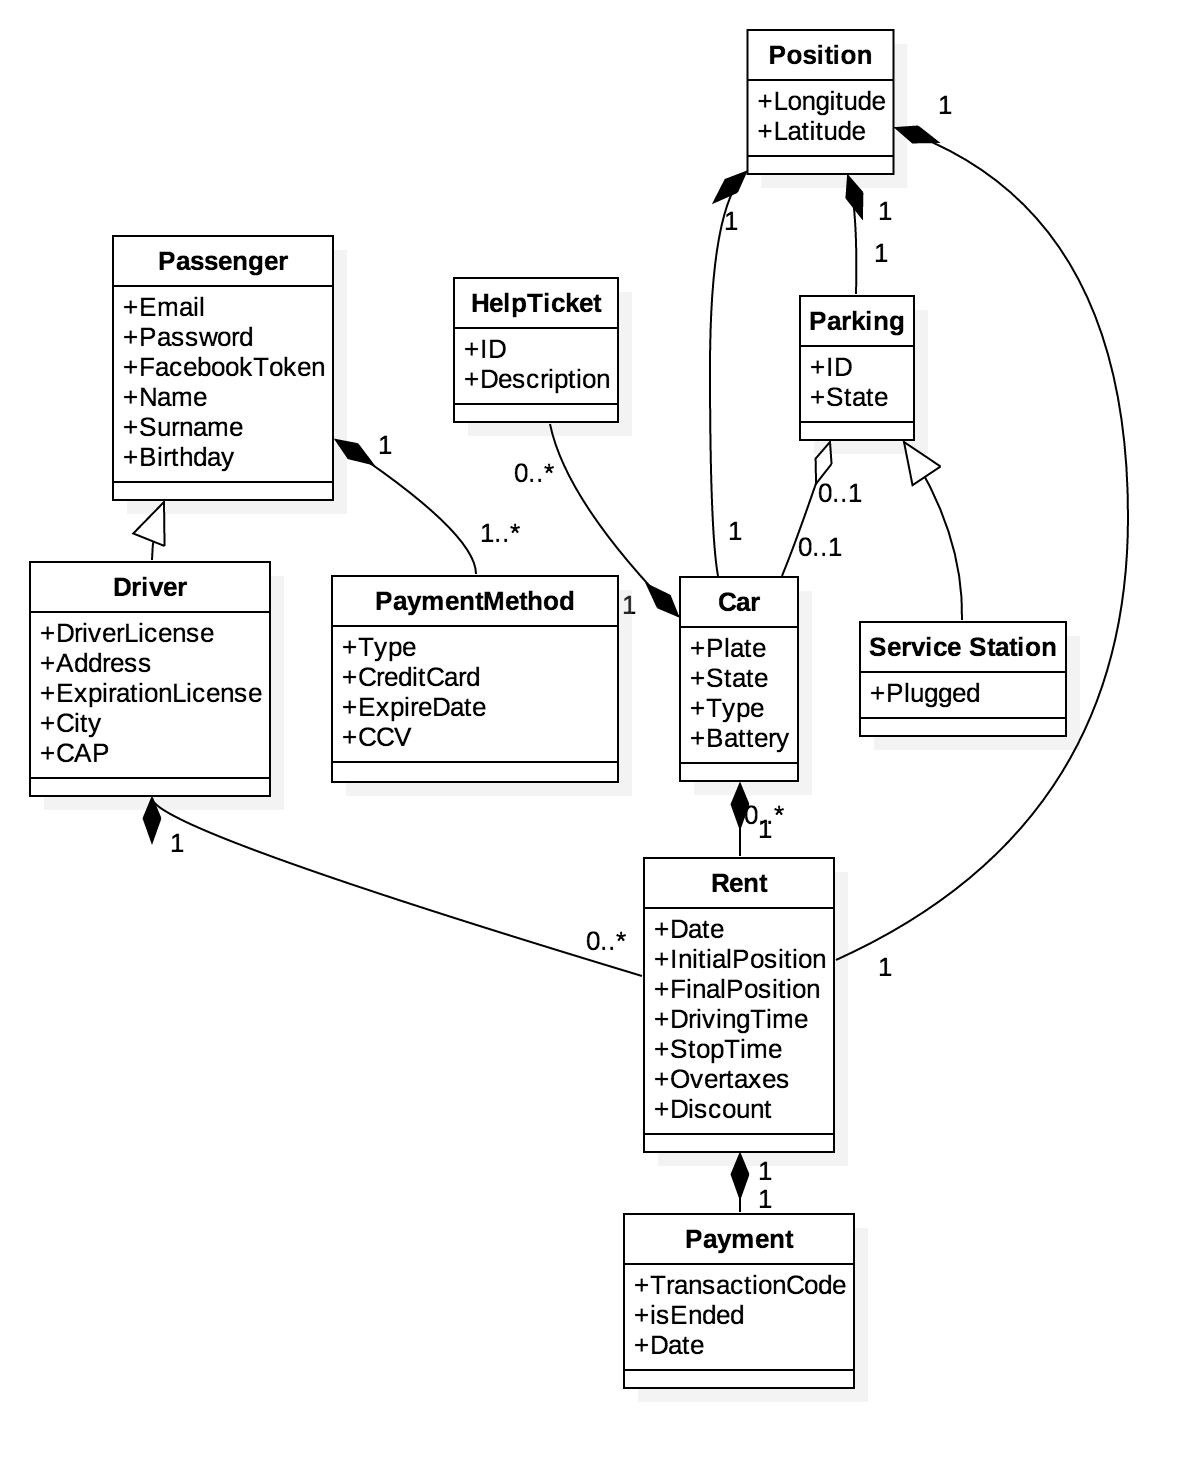
\includegraphics[width=\textwidth]{Resources/UML.png}
    \caption{Class Diagram}
   \end{center}
    \label{fig:ClassDiagram}
\end{figure}
\vfill
\vfill


\section{User characteristics}
The system wants to give to the users an easy way to interact with it. This without undermine the complexity of the problem and achieving all the goal imposted by the stakeholder. To do so, users must be able to install the mobile the application from the store, besides, their phone must be provided with a GPS, a camera and an internet connection.
\section{Constraints}
\subsection{Regulatory policies}
PowerEnJoy is a service provided by a private company. The user, who reaches this service has to agree to License Agreement rather than Privacy policy and Terms of use at registration.\\
The user access and use of the services constitutes his/her agreement to be bound by these Terms, which establishes a contractual relationship between him/her and PowerEnJoy. If user does not agree to these Terms, he/she may not access or use the services. PowerEnJoy may immediately terminate these Terms or any services with respect to him/her, or generally cease offering or deny access to the Services or any portion thereof, at any time for any reason.\\
PowerEnJoy collects the information provided by the user, for example when creating or making changes to services on demand, through contact with customer service or during other communications. This information may include: name, email, phone number, mailing address, payment method, delivery receipts and other information user choose to provide. The personal data will be used only to provide the services requested.\\
User is responsible for obtaining the data network access necessary to use the services. User mobile network's data and messaging rates and fees may apply if he/she accesses or uses the services from a wireless-enabled device. User is responsible for acquiring and updating compatible hardware or devices necessary to access and use the service and applications and any updates thereto.\\
PowerEnJoy does not guarantee that the services, or any portion thereof, will function on any particular hardware or devices. In addition, the services may be subject to malfunctions and delays inherent in the use of the Internet and electronic communications.

\subsection{Hardware limitations}
PowerEnJoy defines the minimum requirements for using web and mobile applications.
\begin{itemize}
	\item \textit{Web application}\\
	See that the web application is a static web site used as advertisement it does not require a minimum access speed and it is built to Browse from Internet explorer 8 or more, intending all the different version of Chrome, Firefox and Safari exit during this time
	\item \textit{Mobile application}\\
	Operating system: Android, iOS, Windows Phone\\
	Memory: 512MB RAM\\
	Hard drive: 40MB of free space\\
	GPS navigation system\\
	Web access at the minimum speed of 1Mbps
\end{itemize}

\subsection{Interfaces to other applications}
PowerEnJoy provides APIs to enable development of additional software on this platform. Furthermore PowerEnJoy manages the communication between itself and the payment management system, to do so the system use the API of the most common payment services used on the web. It is request a system that can work automatically without asking each time the permission to the user. The system sends a payment request with the information of the rent and the amount to pay and the external payment method has to answer with a code that indicate the result of the transaction. Related to the policy of the external system the money that PowerEnJoy earn from the users has to be returned from the payment system no more than a moth after the rent.

\subsection{Parallel operation}
PowerEnJoy supports parallel operations cause of the nature of service. Many users can access to the service at same time thus system and database have to work with parallel requests.

\subsection{Reliability requirements}
PowerEnJoy relies on network connections thus reliability issues are equivalent to performance issues.  However, the application should not corrupt server data as a result of its actions. The system has to guarantee whole-time availability.

\subsection{Criticality of the application}
 PowerEnJoy relies on network systems and servers. Scheduled downtime is acceptable. This system requires a generator backup and redundant power in the event of failover.

\subsection{Safety and security considerations}
PowerEnJoy guarantees secure communications through AES encryption algorithms.
\section{Assumptions and dependencies}
This assumptions are related to the domain and to the environment where the user act.
\begin{enumerate}[label=\subscript{A}{\arabic *}]
 	\item The phone must have a camera and the application must have the right to use it
	\item The user who reserve and/or rent the car is legally responsible for everything that happens during this time
	\item The validity of the payment method is verifiable as the correct end of a payment.
	\item  The car is furnished by some device that allow the system to completely control and communicate with it. As open it from distance, control the passengers number, check its position, check its battery state. 
	\item The user's GPS must be switched on using the mobile app
	\item The user's GPS must work rightly
	\item The users must have a working internet connection
	\item There are a method to charge the battery of the car
\end{enumerate}

\chapter{Specific requirements}
In this chapter are analyzed all the requirements related to the system. Each section corresponds to a specific category of requirement. In particular the section \ref{sec:ExternalInterface} explain the requirements and the constraints the system must to respect to achieve the goal imposed by the customer, as the user interface.
\section{External interface requirements}\label{sec:ExternalInterface}
\subsection{User interfaces}
The interface of PowerEnJoy is done for mobile application (Web is only for the landing page). From figure \ref{fig:LogPage} to figure \ref{fig:CarInfoPage} are presented some of the most important pages and screens of PowerEnjoy. In particular in figure \ref{fig:MapPage} is showed the home page of the PowerEnJoy's application, it is composed by a map and some marker located on the map depending of the position of the car. It's important to understand that only the car in a free state are showed within the map. The figure \ref{fig:CarInfoPage} appears whereas when the user clicks on a marker in the map and shows the information of the selected car and a button to reserve it.
\begin{itemize}
\unbreakableItem{Login Page\\
	\showHeightImage{Resources/LoginMockup.pdf}{Login page}{7cm}{fig:LogPage}
}
\unbreakableItem{Registration page\\
	\showHeightImage{Resources/RegistrationMockup.png}{Registration page}{7cm}{fig:RegistrationPage}
}
\unbreakableItem{Home page or Map page\\
	\showHeightImage{Resources/MapMockup.pdf}{Home page or Map page}{7cm}{fig:MapPage}
}
\unbreakableItem{Car information page\\
	\showHeightImage{Resources/CarInfo.png}{Car information page}{7cm}{fig:CarInfoPage}
}
\end{itemize}
\newpage


\section{System Features}
\subsection{Registration}
Visitors can register to PowEnJoy through mobile application. This operation requires the visitor to fill a registration form with personal data and accept PowEnJoy terms and conditions, including personal data policies, according to local law. The system requires the visitor personal information as name, surname, and birthday, payment information ( as a credit card or a paypal account) and proof of the possesion of a valid driver license.
If any of the previous requirements are not met or any input is invalid, the registration fails and the system asks the visitor to repeat the process. Otherwise, a verification email containing the password of the account is sent to the provided email address. To validate his account the visitor needs to login one time with the provided password.
\paragraphnewline{Use Case} 
\begin{description}
	\item[Name:] User registration
	\item[Actors:] Visitor
	\item[Entry conditions:] There are no entry conditions
	\item[Flow of events:]  \ \\
		\begin{itemize}
			\item The visitor arrives to the home page of the application, as is not logged in ,is redirected to the login/registration page
			\item The visitor enters his personal information, his driver license, a photo of his driver license and some payment method
			\item The visitor clicks on the confirm button
			\item The application suggests the user to read his emails to receive the password
			\item The visitor logs-in after reading the password
		\end{itemize}
	\item[Exit conditions:] The visitor is redirected to the home page of the application
	\item [Exception:] The information furnished by the visitor are not correct or ambiguous as the following case:
		\begin{itemize}
			\item The Email has not format-correct
			\item The Birthday is not at least eighteen years ago
			\item The Payment method is not valid
			\item The informations of the driver license don't correspond with the informations furnished by the visitor
			\item The Driver license is not valid
		\end {itemize}
		Also the visitor could had forgot to enter some requested camps or to accept the Terms and Conditions. In all this case, the system does not send any mail to the visitor but notifies him that an error has been made and allows to input the incorrect data again
	\end{description}

\paragraphnewline{Scenario} \ \\
Meg is a student. She has heard about PowEnJoy and, finding it an easy and ethical way to travel, wants to subscribe to it.
Therefore, she downloads the mobile application from the store and clicks on Register in the main screen. She fulfils the form, accepts the term and conditions  and she click Confirm. However, the system cannot verify Meg's driver license because she forgot to put the photo that prove the possession of it. It therefore asks Meg to take the picture from her mobile's camera. Once she has enter everything correctly she click on Confirm, this time the application valid his credential and tell to Meg to check her emails, she will find the confirmation of the correct registration and the given by the software. Meg read her emails and can finally open the application again and login with the given password and the email she gave before.
\paragraphnewline{Description and Priority} \ \\
This feature is of high priority, it is essential for the system to be.
\paragraph{Functional requirements}
\begin{itemize}
	\item Visitor can abort the registration process at any time.
	\item The password in the email must be used within 1 day, otherwise the registration is deleted along with the visitor's info.
	\item Registration form contain the following information (fields):
	\begin{itemize}
		\item Email address.
		\item First name.
		\item Surname.
		\item Address.
		\item City.
		\item Postal Code.
		\item Credit card code.
		\item Expiration date of the credit card.
		\item Secure code of the credit card.
		\item Driver license code.
		\item Expiration of driver license.
		\item Photo of a driver license.
	\end{itemize}
	\item Email address cannot be the same as ones from other PowerEnJoy users.
	\item The photo of the driver license must be taken by the camera of the mobile.
\end{itemize}
\paragraphnewline{UML Sequence Diagram}
\showPercentImage{Resources/registerSequence.png}{Registration sequence}{1}{fig:regSequence}{0.1em}
\newpage

\subsection{Login}
Visitors on PowerEnJoy mobile application may access to an existing registered user account providing its corresponding email address and password. In case that the submitted info do not match with any existing account info, the system notifies the visitor that the email address doesn't exist, or that it exists, but the submitted password is wrong. In case a user forgets his/her password, the system allows him/her to retrieve it, automatically creating a new password, setting it as the user's one and sending it to the provided email address.
\paragraphnewline{Use Case} 
\begin{description}
	\item[Name:] User Login
	\item[Actors:] User
	\item[Entry conditions:] There are no entry conditions
	\item[Flow of events:]  \ \\
		\begin{itemize}
			\item The user arrives at the Login page of the mobile application.
			\item The user inputs his email address and his password.
			\item The user clicks on the log in button.
			\item The system redirects the user to the home page.
		\end{itemize}
	\item[Exit conditions:] The user is successfully redirected to the application home page.
	\item [Exception:] The email and/or the password furnished by the user are not correct. In this case, the system does not redirect the user to the home page but notifies him that an error has been made and allows to input his email and password again. The user can also forget his/her password, in this case he/she can asks to generate another password and received it on his/her personal email address.
\end{description}
\paragraph{Scenario}
\begin {enumerate}
\item Freddy is user of PowerEnJoy. He has already downloaded the application from the store and he has already done the registration from the application. He cannot remember the password given from the system during the registration time. Therefore he opens the app on the home page and he is redirect to the login page. He click then on the forget password link and the application ask him his email address. He insert the email address and then the application show another message telling the user to check the emails. Once he has received the new password, Freddy can finally open again the application and login with the his email address and the new password.
\item Eleonor is a lawyer familiar with the PowerEnJoy system, she have recently changed phone and she has already download the application again. She open the application and she is redirect in the login page. she fills both fields and clicks on "Log in". The system verifies her info: the operation ends successfully, and she gains access to the user homepage.
\end{enumerate}
\paragraph{Description and Priority}
This feature is of high priority, it is essential for the system to be.
\paragraph{Functional requirements }
\begin{itemize}
	\item Visitors must fill the "email field" with an existing email address in order to successfully log in.
	\item Visitors must fill the "password" field with the only password correspond- ing to the submitted email address in order to successfully log in.
	\item The system will ignore log in requests if at least one of the "email" and "password" fields are left blank.
	\item The system allows visitors to retrieve their password if they forget it, by clicking "Forgot password".
	\item The system requires visitors to submit an existing email address in order to retrieve their password.
	\item The system will take care of assigning the user a new password, when he/she states to have lost the previous one.
	\item The system will take care of sending to the email address submitted by the visitor the new assigned password, when he/she states to have lost the previous one.
	\item The system allows visitors to retrieve their password once a day.
	\item The system remember the user's credential until the user decide to logout.
\end{itemize}
\newpage

\subsection{Reserve car}
Logged user on PowerEnJoy can look for cars near his/her position, or next to a specify address, and reserve one for a rent. This operation is possible using the map on the home page of the application that indicates with a marker the position of the car, only the cars that are in a free state can be reserved and are visible on the map
\paragraphnewline{Use Case} 
\begin{description}
	\item[Name:] Reserve a car
	\item[Actors:] User,
	\item[Entry conditions:] There is at least a car not reserved neither used.
	\item[Flow of events:]  \ \\
		\begin{itemize}
			\item The user arrives at the home page of the application that shows the map with the markers of the cars.
			\item The user choose a car.
			\item The user clicks on the marker of the car chosen.
			\item The user clicks on the "Reserve" button
			\item The application shows to the user the time remained to start the engine and the position of both the actors.
			\item The user arrives next to the car.
			\item The user clicks on the button "Open the car"
			\item The car is opened by the system
			\item The user get into the car and start the engine.
		\end{itemize}
	\item[Exit conditions:] The user successfully start the engine of the car
	\item [Exception:] Two users reserve the same car in a really small difference of time, the system in this case will delete the reservation that is requested later.
\end{description}
\paragraphnewline{Scenario} \ \\
Francis needs to go home from a dinner with his friends. It is late and there are public transport anymore. He is already registered and successfully logged-in in the PowerEnJoy application. He decided to reserve a car using the application. He opens the application and he is directly redirect to the application home page that contains the map with the markers of cars near him. He chooses a marker and he click on it. The app shows him the information of the car as its battery charge and its position. The car is really close to him therefore he clicks on the button reserve and he moves next to the car. Meanwhile the application shows him the  a timer, the vehicle registration plate, his position and the position of the car. Once the Francis arrives next to the car the app shows him a button to open the car. The rent starts when Francis starts the engine of the car.
%Another scenario with a men who can't reach the car until in one hours?
\paragraphnewline{Description and Priority} \ \\
This feature is of high priority, it is essential for the system to be.
\paragraph{Functional requirements }
\begin{itemize}
	\item A car changes is state from \emph{"Reserved"} to \emph{"In use"} only when the engine starts
	\item A car can be reserved and showed on the map only if its state is \emph{"Free"}
	\item A car stays in the \emph{"Reserved"} state for at maximum one hour, if it's not picked-up it return to the state \emph{"Free"}
	\item Each car have a precise position
	\item An user can open the car through the app only if it is near to it
	\item Each user can reserve only one car at the same time
	\item A car can be reserved from only one user at the same time
\end{itemize}
\paragraphnewline{UML Sequence Diagram}
\showPercentImage{Resources/bookSequenceDiagram.png}{Car reservation}{1}{fig:bookCarSequence}{0.1em}

\subsection{End a rent}
Once the user has finished his/her ride he/she have to park the car in a safe area or a parking, stop the engine and get off the vehicle. The system checks if all the requirements to end the rent are respected and closes the car. The system waits 5 minute to let the user plug the car if he/she wants to. After the wait of time the system sends the payment request to the external payment system. The end of a rent can also provide some discount on the final payment or the add some overtaxes.
\paragraphnewline{Use Case} 
\begin{description}
	\item[Name:] End a rent
	\item[Actors:] User, Car
	\item[Entry conditions:] The car is in the state In Use
	\item[Flow of events:]  \ \\
		\begin{itemize}
			\item The user stop the engine of the car and get out of the vehicle.
			\item The car check if all the doors are closed and there is no one into the it.
			\item The system close the car
			\item The system wait 5 minute
			\item The system send the request for payment to the external system
			\item The external system answer to the request
			\item The system notify the user about the end of the rent with a message on the app
		\end{itemize}
	\item[Exit conditions:] The user successfully ends the rent
	\item [Exception:]
		\begin{itemize}
			\item The car is not parked in predefined area, in this case the system will not allow the user to end rent and close the car.
			\item The payment request failed, in this case the system blocks the user and he/her will not be able to use the system  again until he complete the payment
			\item The car is stopped but the user still inside or a door is open, in this case the rent will not end and the user is charged as he/she would still driving.
		\end{itemize}
\end{description}
\paragraphnewline{Scenario} \ \\
\begin{enumerate}
	\item Isa is an habitual user of PowerEnJoy. She picked-up a car to cross the city and be ecologic with the system. She has finished her ride and she wants to end the rent. She parks the car near a safe area near her destination and she stops the engine of the car. The safe area, as defined, has a plug to recharge the car so Isa plugs the car just after she has stopped the car. The system notify Isa of the correct end of her rent and show her the final bill, that contain a discount of 30\%, with a message on the application.
	\item Laura took a car of PowerEnJoy to get home with her family, her husband and her tow child. She park the car in a parking but unfortunately the battery of the car is at 10\% and there are no safe area next to Laura's house, the most near is 3.2 Km away. Laura end her rent stopping the engine of the car and receives a message from the app that shows her an overtaxes of 30\% due to the position of the parking and the state of the battery life of the car.
	\item Mary rented a car to go home from her university, once she arrives next to her destination she park the car into a parking, she stop the engine and get off the car. Unfortunately the chosen area is not an allowed parking area and the system does not let the her close the car even if nobody is into it. Therefore she moves the car into another parking area and this time, once she followed the procedure, the system close the vehicle and wait 5 minute before charging Mary for her rent. Once the payment is successfully ended the system send a notification to Mary with the resuming of her rent and the bill.
\end{enumerate}
\paragraphnewline{Description and Priority} \ \\
This feature is of high priority, it is essential for the system to be.
\paragraph{Functional requirements }
\begin{itemize}
	\item If the system detects the user took at least two other passengers into the car, the system applies a discount of 10\% on the last ride.
	\item If a car is left with no more than 50\% of the battery empty, the system applies a discount of 20\% on the last ride.
	\item If a car is left at special parking areas where they can be recharged and the user takes care of plugging the car into the power grid, the system applies a discount of 30\% on the last ride.
	\item If a car is left at more than 3 KM from the nearest power grid station or with more than 80\% of the battery empty, the system charges 30\% more on the last ride to compensate for the cost required to re-charge the car on-site.
	\item The user has five minutes to plug the car if he/she wants a discount
	\item The rent end-up only if the car is closed, parked in a parking/safe area and there is anybody in the vehicle.
	\item The car can be closed only if it is turned off, there is no one in it and if it is parked into a safe/parking area
	\item The discount can be apply only if there are not any overtaxes
	\item Only one discount can be apply to the rent, the one who is the most convenient for the user.
	\item The user has 2 minute before the check of the requirements condition
\end{itemize}
\paragraphnewline{UML Sequence Diagram}
\showImage{Resources/endRent.png}{End rent sequence}{fig:endSequence}
\showImage{Resources/Payment.png}{Payment sequence}{fig:paymentSequence}
\newpage

\subsection{Report problems}
Every logged-in user can report a problem to the PowerEnJoy team during the all time of use of the system. In particular the user has a button to immediately contact the customer service during:
\begin{itemize}
	\item The reservation of a car, in case the car is not opened by the system.
	\item The rent of a car, in case of accident or problem due to the system.
	\item The charge of a car, in case some safe area is not working correctly.
	\item The payment, in case of some error appeared during the payment time.
\end{itemize}
\paragraphnewline{Use Case} 
\begin{description}
	\item[Name:] Report problems
	\item[Actors:] User, External Customer service
	\item[Entry conditions:] The user needs to be logged into the application and some part of the system must have a malfunction.
	\item[Flow of events:]  \ \\
		\begin{itemize}
			\item The user clicks on the button help in the menu of the application
			\item The phone automatically call the customer service 
			\item A customer service operator answer to the user and help him/her to solve the problem or open a repair request on the car
		\end{itemize}
	\item[Exit conditions:] The user successfully resolve or notify the problem
	\item [Exception:] The information furnished by the user are not correct or ambiguous and the operator cannot help the user solving his/her problem. In this case if the operator will notify to the external system a reparation needed. The user have no credit in the phone to call the customer service, in this case the app will call the service through the internet connection 
\end{description}
\paragraphnewline{Scenario} \ \\
\begin{enumerate}
	\item Marc is a logged user who has already reserved a car. The rented car is really near to him and Marc wants to open it. Unfortunately the board computer of the chosen car, the one that able the system to open it, it is broken.Therefore he decides to call the customer service with the button in the reservation page. The customer service office answer to his call and let Marc abort his reservation without paying any additional feeds.
	\item Claire is a user of PowerEnJoy who is renting a car, during her ride she rear-end another vehicle. Unaware about the procedure to follow she open the PowerEnJoy application and she click on "Customer service" in the menu. An employ of PowerEnJoy system answers and explains all the document Claire needs to complete before end her rent with the procedure to follow in her case. The operator opens also a Intervention request with the third-part company who is responsible to maintain and repair the cars of the system.
	\item Jack is using a PowerEnJoy's car and he wants to park it because he is near to his destination. The battery charge is under 20\% and he wants to plug the car in charge in order to let the next user able to use it for a longer period of time. Unfortunately the nearest safe area is broken and Jack cannot plug the car into charge. To not income in overtaxes he decides to call the Customer service. The employ answers to Jack's call and report the problem to the third-part agency. In plus the PowerEnJoy employ preserve Jack to receive overtaxes on his last rent but he also block every type of discount.
\end{enumerate}
\paragraphnewline{Description and Priority} \ \\
This feature is of medium priority, it is not essential for the system to be.
\paragraph {Functional requirements }
\begin{itemize}
	\item The user must be able to contact the customer service 24h/24h
\end{itemize}
\paragraphnewline{UML Sequence Diagram} \ \\
\showImage{Resources/reportProblem.png}{Report problem sequence}{fig:reportProblemSequence}
\newpage

\subsection{Profile settings}
The system allows logged in users to view and modify their profiles at any moment, as long as they are logged in. While modifying email addresses, driver license or payment method must be unique in all the system, otherwise the system denies the modification request. In case of modify of email address, the system sends a confirmation email to the new address. Modification will successfully ends when the user clicks the link in the sent email.
\paragraphnewline{Use Case} 
\begin{description}
	\item[Name:] Profile settings
	\item[Actors:] User
	\item[Entry conditions:] The user needs to be logged into the application
	\item[Flow of events:]  \ \\
		\begin{itemize}
			\item The user clicks on profile in the menu of the application
			\item The user changes his/her information that have changed
			\item The system notifies the user that the settings have been successfully updated.
		\end{itemize}
	\item[Exit conditions:] The user successfully saves his/her new settings
	\item [Exception:] The information furnished by the user are not correct or ambiguous as the following case:
		\begin{itemize}
			\item The Email has not the correct format
			\item The Birthday is not at least eighteen years ago
			\item The Payment method is not valid
			\item The information's of the driver license don't correspond with the information furnished by the visitor
			\item The Driver license is not valid
		\end {itemize}
\end{description}
\paragraphnewline{Scenario} \ \\
\begin{enumerate}
	\item  Zac periodically changes his account password, in order to increase protection. To do so, every 3 months, he opens PoweEnJoy on his mobile phone, chooses "Profile", then "Modify". He selects the password field, writes down a new one, then writes it again in the "Confirm password" field. Finally, he clicks "Confirm": the system informs him that his account password has successfully been updated.
	\item Sailor is a user of PowerEnJoy and she has recently change her credit card because it was expired. She needs so to open PoweEnJoy on his mobile phone, chooses "Profile", then "Modify". She selects the old credit card and she writes all the new information about her new payment method. Finally she clicks "Confirm" and the system informs her that the account payment has been successfully updated.
\end{enumerate}
\paragraphnewline{Description and Priority} \ \\
This feature is of low priority, it is not necessary but it is a service to create a better user expirience.
\paragraph{Functional requirements }
\begin{itemize}
	\item Account settings are accessible from the start screen of both apps, through the "Profile" button.
	\item The system allows users to view all their profile info, submitted during registration
	\item The system allows users to modify all their profile info, submitted during registration.
	\item Modifying the password requires to write the old one, and the new one twice; if the former password is not correct or if the two new passwords submitted do not match, the system asks for all passwords again and notifies the user.
	\item Modifying the email address, the driver license requires that the new one doesn't match with the one of another registered user.
	\item Modifying the email address requires confirmation through an email sent to the submitted email address.
	\item The system allows users to abort modifications at any time.
	\item The system allows users to delete their account: confirmation is required to proceed.
\end{itemize}
\newpage

\section{Alloy}
In this section is presented the alloy model with its execution results
\alloyfile{./Alloy/PowerEnJoy.als}
\newpage

\subsection{Alloy Model Execution Results}
\begin{itemize}
	\itemBold{Alloy Console}\\
		\showImage{Resources/alloyConsole.png}{Alloy Console.}{fig:mdlConsole}\newpage
	\itemBold{Alloy Simple World}\\
    \showPercentImage{Resources/SimpleWorld.pdf}{Alloy Simple World.}{0.9}{fig:simpleWorld}{0.5em}\newpage
	\itemBold{Alloy Real World}\\
    \showPercentImage{Resources/RealWorld.pdf}{Alloy Real World.}{0.5}{fig:realWorld}{0.1em}\newpage
\end{itemize}


\section{Performance Requirements}
%TODO
PowerEnJoy will perform 95\% of the operations within 4 seconds; the total amount of the operations within 10 seconds.
The system should ensure at least 2000 passangers connected.

\section{Design constraints}
PowerEnJoy wants to reach most of users, requiring minimum specifications for devices.
User, registered to the system, have to use their own devices provided with GPS navigation system to perform the service. Mobile applications have to offer backward compatibility.

\section{Software system attributes}
\paragraph{Reliability}
The mean time between failures (MTBF) shall exceed 3 months.
\paragraph{Availability}
In order to maintain the system up-to-date and secure, PowerEnJoy schedules downtime periods where will be executed routine operations. The service should be available 99\% of the time.
\paragraph{Security}
myTaxiService to ensure service availability and data protection use:
\begin{itemize}
	\item AES cryptography algorithm on network operations
	\item Data are encrypted and stored in backup drives to prevent system failure
	\item Login authentication. Users, after the registration, have to confirm their e-mail with the security code sent to the e-mail write in the registration form
	\item SQL injection detection
\end{itemize}
Server architecture will be implemented separating
data from application. Application server must be separated
from database and from the web server. All architectures are divided by firewalls.
\paragraph{Maintainability}
To ensure an easy maintenance of the software, it must be well-documented and written following coding patterns.
\paragraph{Portability}
Web programming ensures a wide target of browser. Mobile applications instead, cause of different languages and devices, have to be written following coding patterns for easy portability.
Availability of the service is ensured by hardware and software limitations in Section 2.4.2.



\appendix
\chapter{Appendix}

\section{Tools}
\begin{itemize}
	\itemBold{TeXstudio} \LaTeX{} editor used to write the document.
	\itemBold{Alloy Analyzer 4.2} Used to build an Alloy Model and to check its consistency.
	\itemBold{StarUML} Used to build UML Class Diagram and UML Use Case Diagrams.
	\itemBold{draw.io WebSite} Used to design the UML Sequence Diagram and the Mockup (wep portal and smartphone app).

\end{itemize}
\newpage
\section{Hours of work}
In the following are listed the hours of work that each member of the group did:
\begin{enumerate}
	\item Marco Redaelli: 41 \emph{hours}
	\item Francesco Zanoli: 41 \emph{hours}
\end{enumerate}
\newpage
\section{Version History}
In the following are listed the differences between versions:
\begin{enumerate}
	\itemBold{13/11/2016} First version
	\itemBold{11/12/2016} Requirement enumeration changes, Edit version' table
\end{enumerate}

\end{document}
